% ----------------------------------------------------------
% Apêndices
% ----------------------------------------------------------

% ---
% Inicia os Apêndices
% ---
\begin{apendicesenv}

% Imprime uma página indicando o início dos Apêndices
\partapendices

% ----------------------------------------------------------
\chapter{Vídeos demonstrando o rastreio pelo sistema simulado no software MuJoCo}\label{cap:apendice_umbra}
% ----------------------------------------------------------

Para exemplificar o funcionamento do protótipo, foi desenvolvido um modelo simulado no software MuJoCo (discutido no capítulo \ref{sec:MuJoCo}).
O primeiro vídeo pode ser encontrado na referência \cite{youtube_umbra} e na Figura \ref{fig:QR_Umbra} e contém uma demonstração do sistema rastreando o satélite Umbra-07.

\begin{figure}[htbp]
    \centering
    
\includegraphics[width=0.5\textwidth]{figs/QRCODE_passagem_umbra.png}
    \caption{Código QR do vídeo do sistema rastreando o satélite Umbra-07}
    \legend{Fonte: Autor(2026)}
    \label{fig:QR_Umbra}
\end{figure}

Em 3:55, é possível observar o aumento da velocidade da passagem quando o satélite se aproxima de elevações mais altas.
O Umbra-07 atinge a sua maior elevação em 5:02, quando inicia a reduzir a elevação em relação à antena.
A passagem é finalizada em 10:57, no qual a elevação do satélite chega a zero e o sistema retorna à sua posição de origem.

\begin{figure}[htbp]
    \centering
    
\includegraphics[width=0.5\textwidth]{figs/QRCODE_troca_satelites.png}
    \caption{Código QR do vídeo do sistema rastreando o satélite Umbra-07}
    \legend{Fonte: Autor(2026)}
    \label{fig:QR_Troca_Sats}
\end{figure}

O segundo vídeo é referente ao filtro lidando com troca de satélites alvo, presente na referência \cite{youtube_troca_satelite} e no Código QR da Figura \ref{fig:QR_Troca_Sats}.
O vídeo se inicia com o usuário selecionando o satélite COSMOS 2561 a ser rastreado utilizando o SatDump.
Em 0:06, o sistema é acionado e a antena é alinhada com o satélite, aproveitando a primeira volta do sistema.
Em 0:34, o satélite KUIPER-00183 é selecionado e a antena inicia o novo rastreio.
O envio do rastreio é desabilitado em 1:20, e é possível perceber o sistema divergindo da posição real.

Em 1:51, o sistema para de rastrear o ONEWEB-0399 e começa a rastrear o satélite YAOGAN-30 05C, sendo possível verificar o sistema oscilando para se corrigir à nova órbita.
O sistema se estabiliza por volta de 2:12, conseguindo rastrear a nova trajetória.
Em 2:46, o algoritmo verifica que não está recebendo mais informações do satélite e retorna à sua posição inicial, mas logo inicia o rastreio do KSM1-C.
A troca do rastreio do KSM1-C para o 2024-205G em 3:05 provoca uma outra oscilação no sistema enquanto o filtro captura as informações da nova órbita.

A alteração do ONEWEB-0095 para o CE-SAT-IE em 3:40 demonstra que o filtro não sofre muitas oscilações quando as trajetórias são próximas.
Em 4:55, há uma demonstração do filtro quando este recebe duas trajetórias próximas, mas com direções distintas, provocando oscilações em azimute e elevação.
Em 5:21, o sistema passa por um \textit{wrap} do azimute, quando o algoritmo precisa lidar com uma transição de $360^{\circ}$ para $0^{\circ}$ durante a passagem do KSM1-C.

É possível ver o sistema divergindo quando desengajado durante o rastreio do ASRTU-1 (AO-123) até o momento que este entra em sua rotina para retornar à volta inicial simulando o desenrolar dos fios do sistema em 6:57.
O satélite STAR ONE C2 é rastreado em 7:00, sendo este um satélite geoestacionário.
Em 8:28, novamente o \textit{wrap} do azimute é demonstrado ao desengajar um sistema que estava próximo de $0^{\circ}$ (METOP-C) e rastreando um satélite próximo de $360^{\circ}$ (SCD 2).
Em 8:45, é possível perceber o que ocorre quando há uma interrupção no rastreio em uma região onde a trajetória sofre grande aceleração (por estar próxima ao zênite), mostrando que o sistema diverge rapidamente da rota original, tanto em azimute quanto em elevação.
O sistema realiza mais um retorno à posição inicial em 9:39 e permanece por mais tempo sem receber dados, posicionado com valores de azimute e elevação igual a zero e em 10:08 o sistema é completamente desligado das informações do aplicativo até o vídeo terminar.

% ----------------------------------------------------------
\chapter{Levantamento de Parâmetros do Filtro SAWBird+ GOES}\label{cap:apendice_filtro_saw}
% ----------------------------------------------------------
Segundo a folha de dados do filtro SAWBird+ GOES \cite{nooelec_sawbird_goes}, seu ganho máximo é da faixa de $38 \text{ dB}$ em $1694 \text{ MHz}$ com uma potência máxima de saída de $20 \text{ dBm}$ e uma largura de banda de $70 \text{ MHz}$.
Sabendo disso, foi utilizado um gerador de RF configurado para a frequência de $1,7 \text{ GHz}$ e amplitude de $-25 \text{ dBm}$. Para testar que o gerador estava com a configuração correta em sua saída, foi utilizado um analisador de espectro para medir a potência recebida.
Com a validação da configuração do experimento correta, com amplitude de $-25,2 \text{ dBm}$ (visto na Figura {\ref{fig:saw_gerador_conec_direta_visor}}), o filtro SAW foi conectado na linha de transmissão (veja Figura \ref{fig:setup_filtro_desligado_total}).
Assim como o esperado, o filtro desligado faz com que o sinal passante não seja muito maior que o piso de ruído do sistema, porém com uma pequena passagem do sinal ainda visível (vide Figura \ref{fig:setup_filtro_desligado}).

O amplificador é então ligado através de sua entrada USB-C para verificar o ganho de seu circuito ativo (Figura \ref{fig:setup_filtro_ligado}).
É esperado um ganho próximo ao teórico, calculado pela diferença entre a potência de entrada com o filtro ligado e com a saída do gerador.
Para o experimento, a saída do filtro ativo tem o ganho de $12,6 \text{ dB}$ (veja Figura \ref{fig:setup_filtro_ligado_visor}), fazendo com que o ganho total seja de $G_{dB} = 12,6\text{ dBm} - (-25\text{ dBm}) = 37,5 \text{ dB}$, que é próximo do valor máximo descrito na folha de dados.

Para o cálculo da banda de passagem, foi alterada a frequência do gerador até encontrar uma região que tenha um ganho de $-3 \text{ dB}$ abaixo do ganho máximo do sistema, que seria aproximadamente $9,6 \text{ dBm}$.
A região equivalente à banda inferior foi encontrada quando a frequência estava por volta de $1653 \text{ MHz}$ (vide Figura \ref{fig:filtro_saw_banda_baixa}), enquanto a maior frequência da banda foi encontrada em $1724 \text{ MHz}$ (conforme observado na Figura \ref{fig:filtro_saw_banda_alta}).
A largura de banda do filtro é calculada como sendo de $BW = 1724 - 1653 = 71 \text{ MHz}$, que é bem próxima da banda estabelecida pela folha de dados. Além disso, é possível determinar a frequência central do filtro como sendo de $f_{c} = \frac{1724+1653}{2} = 1688,5 \text{ MHz}$, estando bem próximo à frequência especificada.

Assim, é possível dizer que o filtro está se comportando de maneira nominal aos parâmetros designados pela empresa fabricante, garantindo que este funcione conforme o esperado.

\begin{figure}[htbp]
    \centering
    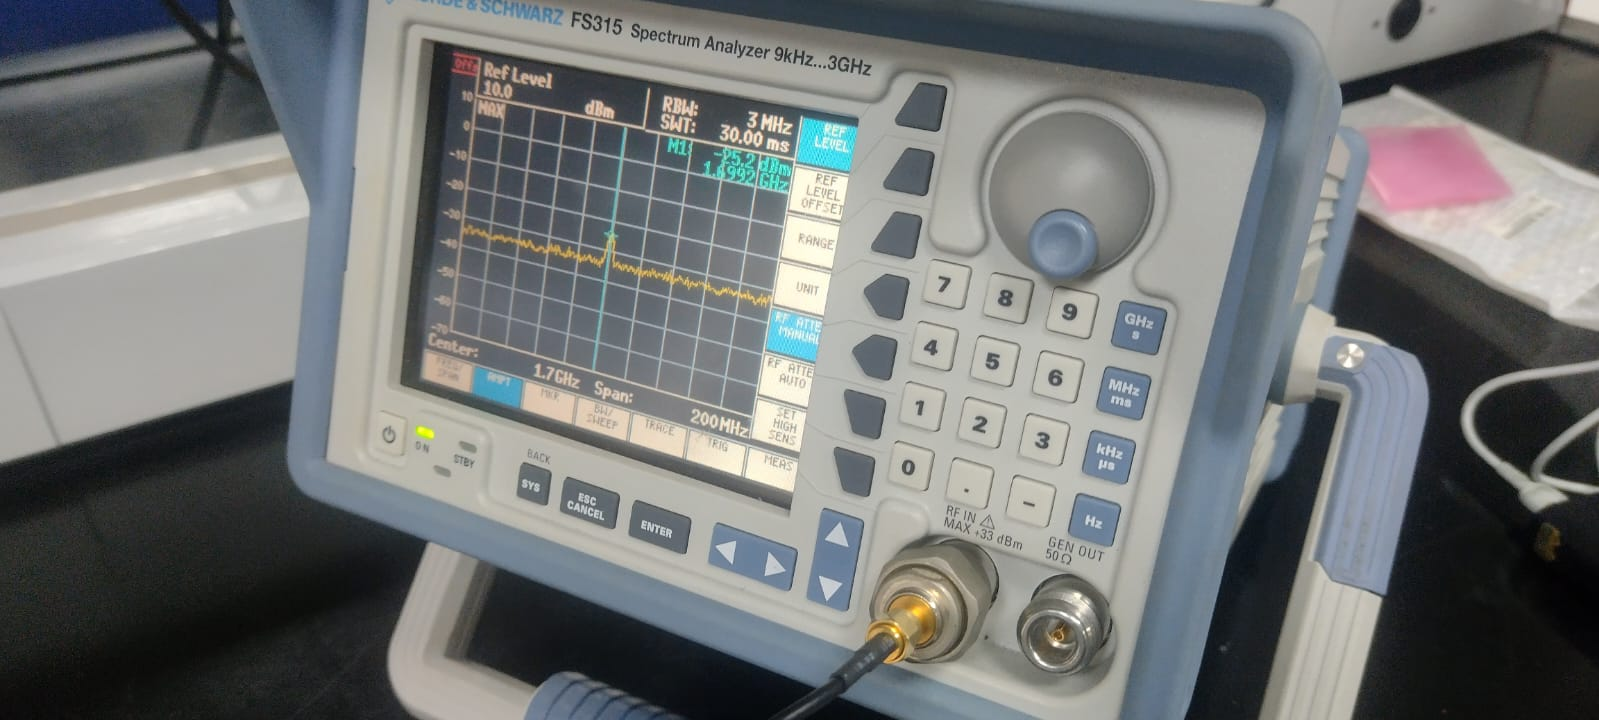
\includegraphics[width=1\textwidth]{figs/conec_direta_gerador_visor.jpeg}
    \caption{Foto do sinal observado no analisador de espectro quando o gerador foi conectado diretamente à entrada.}
    \legend{Fonte: Autor(2026)}
    \label{fig:saw_gerador_conec_direta_visor}
\end{figure}
\begin{figure}[htbp]
    \centering
    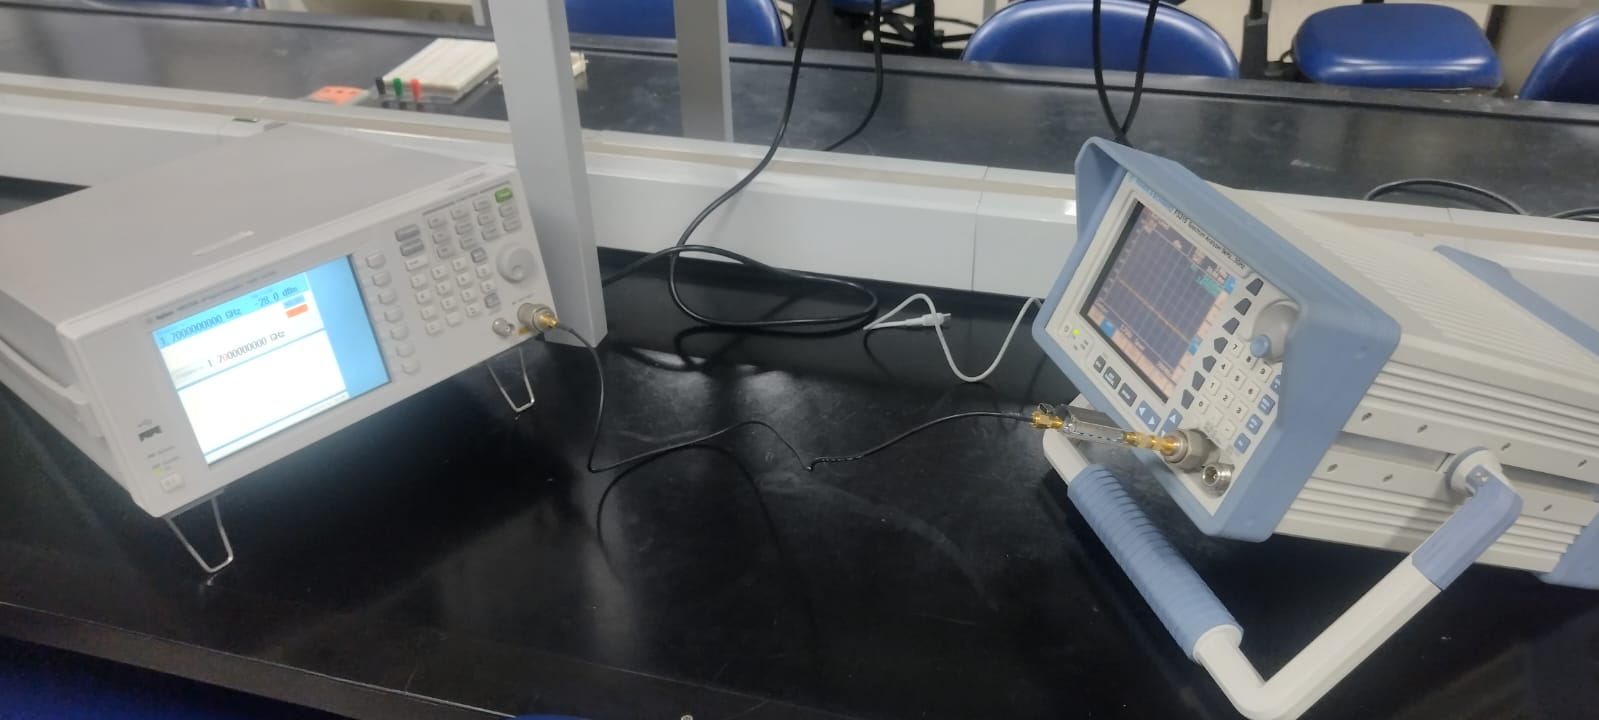
\includegraphics[width=1\textwidth]{figs/setup_filtro_desligado_total.jpeg}
    \caption{Configuração de gerador, analisador e filtro SAW desligado.}
    \legend{Fonte: Autor(2026)}
    \label{fig:setup_filtro_desligado_total}
\end{figure}
\begin{figure}[htbp]
    \centering
    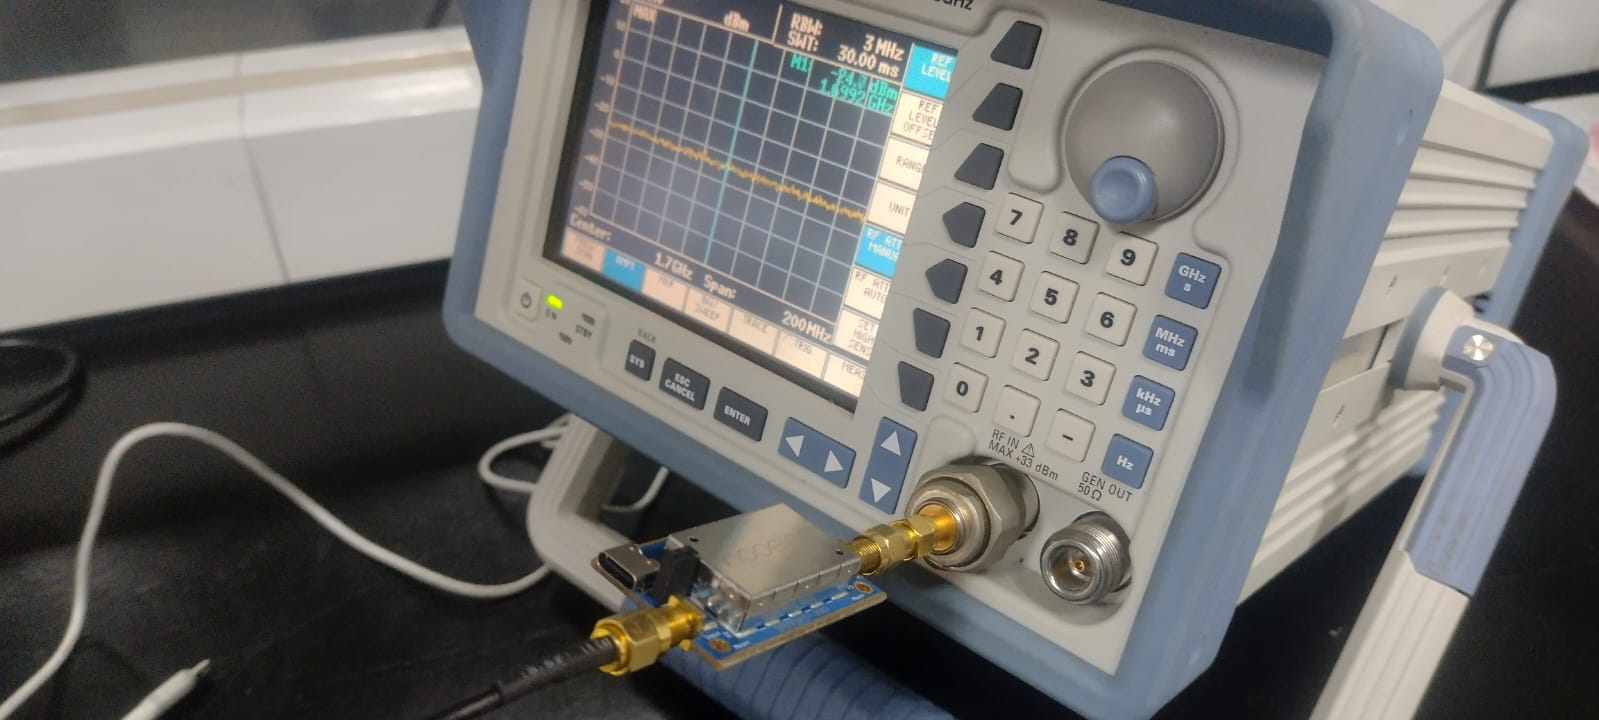
\includegraphics[width=1\textwidth]{figs/setup_filtro_desligado.jpeg}
    \caption{Medição do sistema com o filtro SAW desligado.}
    \legend{Fonte: Autor(2026)}
    \label{fig:setup_filtro_desligado}
\end{figure}
\begin{figure}[htbp]
    \centering
    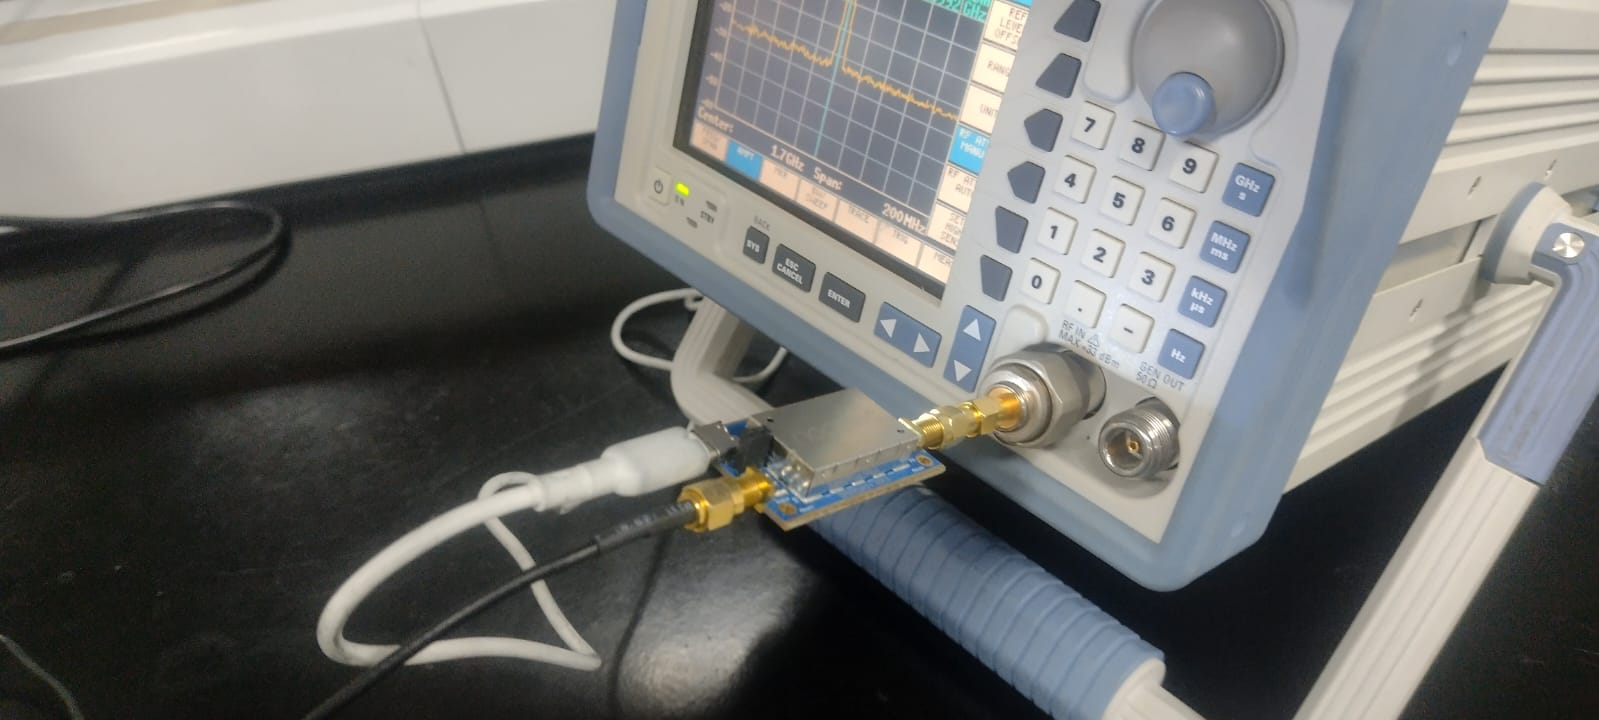
\includegraphics[width=1\textwidth]{figs/setup_amplificador_ligado.jpeg}
    \caption{Filtro ligado por USB-C.}
    \legend{Fonte: Autor(2026)}
    \label{fig:setup_filtro_ligado}
\end{figure}
\begin{figure}[htbp]
    \centering
    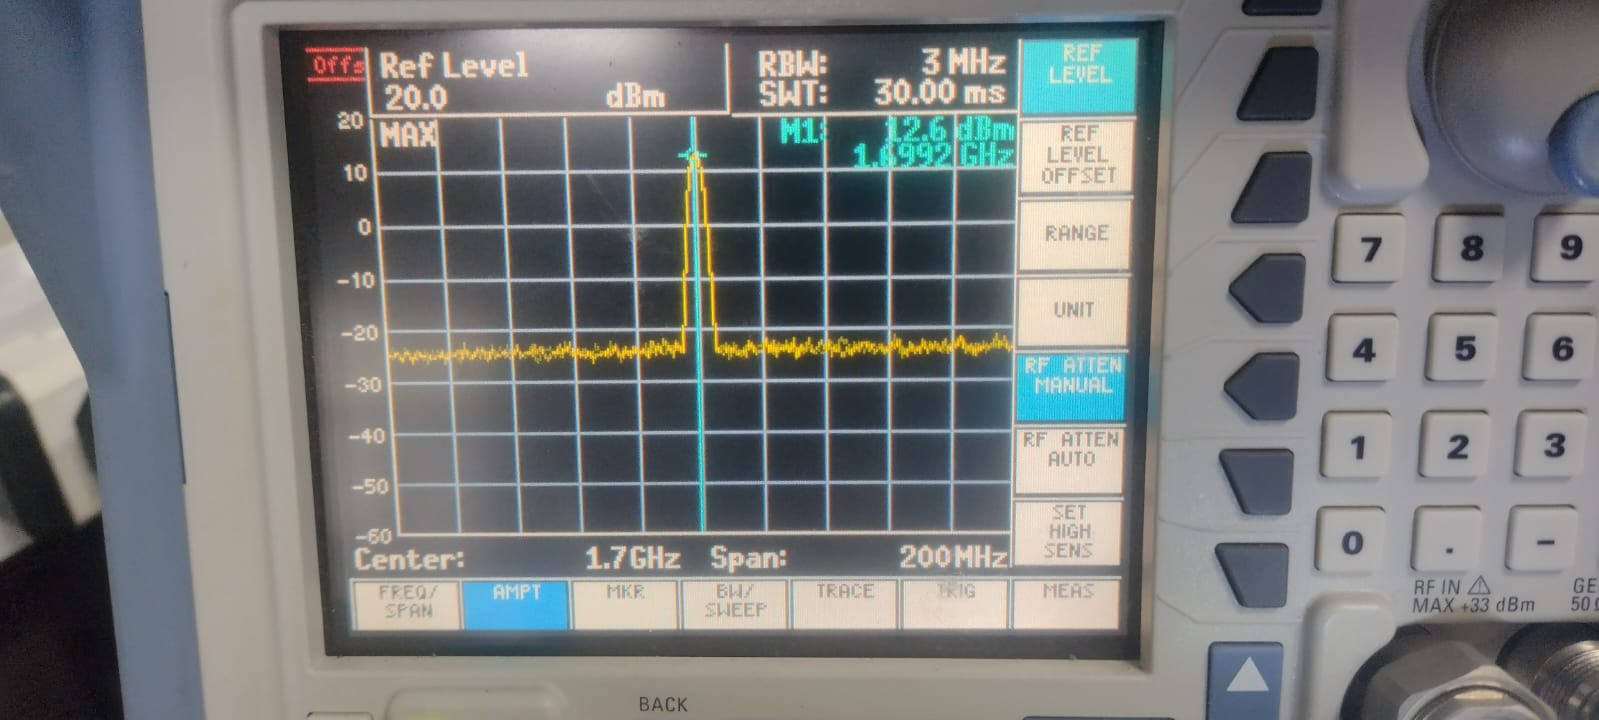
\includegraphics[width=1\textwidth]{figs/visor_amplificador_ligado.jpeg}
    \caption{Medição para o amplificador ligado em $1,7 \text{ GHz}$.}
    \legend{Fonte: Autor(2026)}
    \label{fig:setup_filtro_ligado_visor}
\end{figure}
\begin{figure}[htbp]
    \centering
    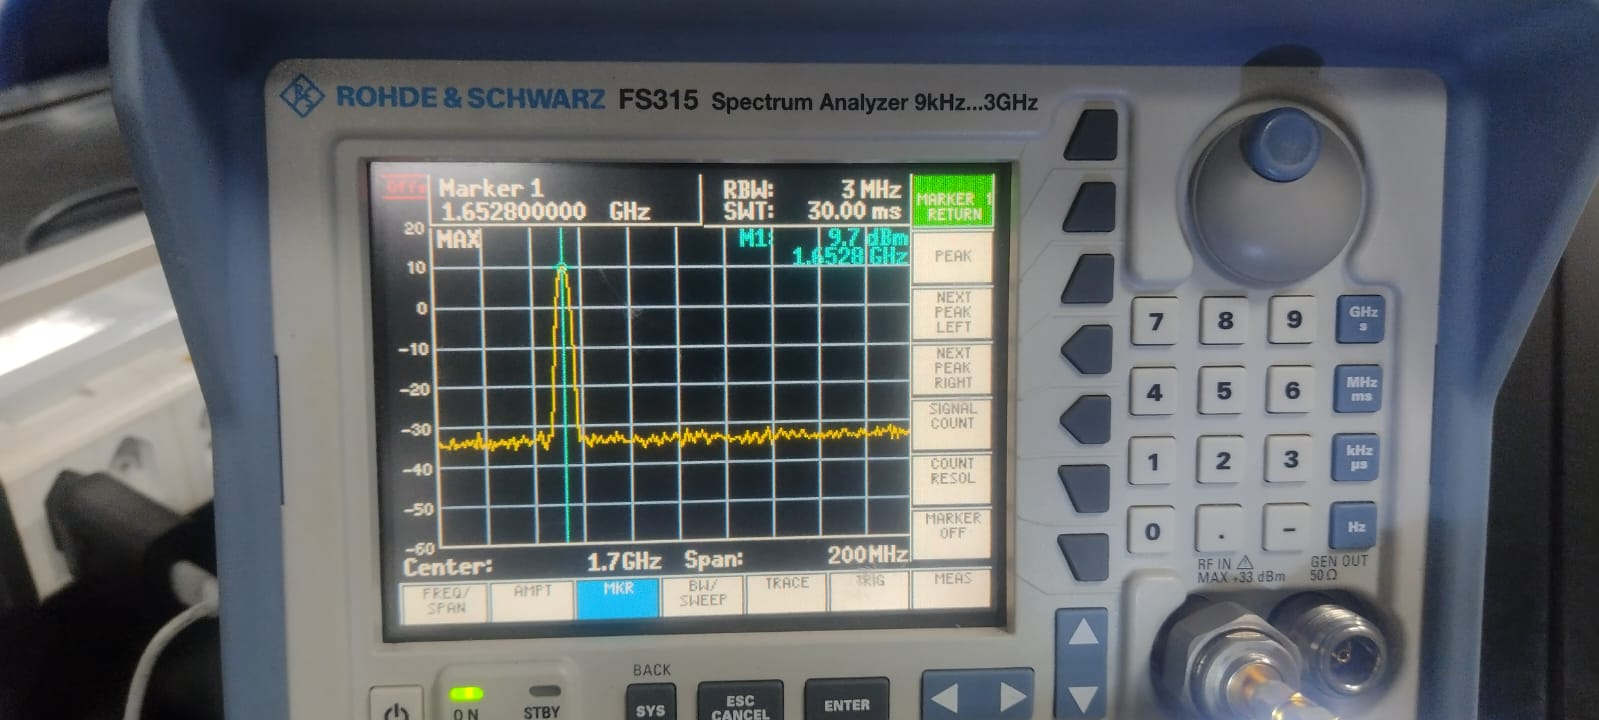
\includegraphics[width=1\textwidth]{figs/filtro_banda_baixa.jpeg}
    \caption{Medição para o amplificador ligado para sua banda inferior, de $1653 \text{ MHz}$.}
    \legend{Fonte: Autor(2026)}
    \label{fig:filtro_saw_banda_baixa}
\end{figure}
\begin{figure}[htbp]
    \centering
    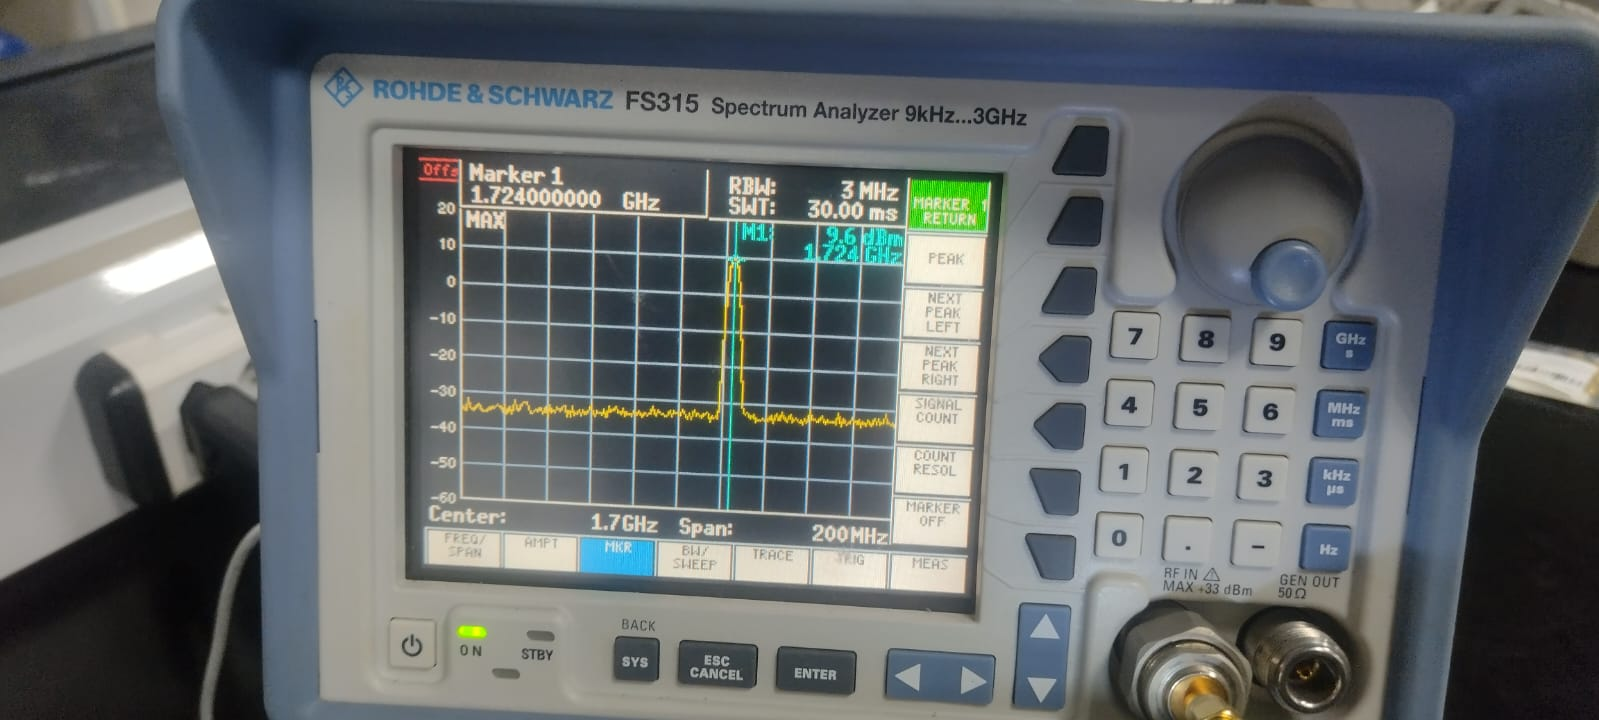
\includegraphics[width=1\textwidth]{figs/filtro_banda_alta.jpeg}
    \caption{Medição para o amplificador ligado para sua banda superior, de $1724 \text{ MHz}$.}
    \legend{Fonte: Autor(2026)}
    \label{fig:filtro_saw_banda_alta}
\end{figure}
% ----------------------------------------------------------
\chapter{Levantamento do Padrão de Radiação da Antena Helicone}\label{cap:apendice_teste_diagrama radiação}
% ----------------------------------------------------------
Para o teste realizado, os equipamentos utilizados foram: gerador de frequência de RF; analisador de espectro; antena helicone (confeccionada para este trabalho); antena Yagi projetada em uma PCB; e filtro SAWBird+ GOES.
Como ferramentas, foram utilizados um tripé de câmera, um barbante, e um transferidor. As conexões foram feitas utilizando cabos SMA-SMA e adaptadores SMA-N para o encaixe nos equipamentos. Todos os equipamentos podem ser vistos na Figura \ref{fig:todos_equipamentos_diagrama_radiacao}.

O gerador de RF foi configurado para a frequência de $1,7 \text{ GHz}$ e potência de $-30 \text{ dBm}$ (veja Figura \ref{fig:config_gerador_filtro}). O amplificador foi ligado para amplificar a saída do sinal, pois o gerador não estava mantendo sua saída constante acima de $-20 \text{ dBm}$.
Os suportes das antenas foram ajustados para se manterem no mesmo plano horizontal, garantindo que a seção do plano vertical da antena estivesse centralizada na antena de teste (conforme demonstrado na Figura \ref{fig:alinhamento_antena_plano_horizontal}).
Após isso, foi feita uma medição desde a região mais distante da antena até o dipolo da antena Yagi (\ref{fig:medicao_dist_antenas}). A distância entre os elementos é de aproximadamente $57 \text{ cm}$, que é maior que a distância de campo distante discutida no Capítulo \ref{sec:antena}.

O experimento iniciou na medida de $90^{\circ}$ do transferidor (que posteriormente foi subtraída do ângulo medido).
A movimentação horária da Yagi em relação à direção traseira para a frontal da helicone representa seu lado direito, enquanto a movimentação anti-horária representa seu lado esquerdo.
O lado direito foi considerado como ter angulação negativa, enquanto o lado esquerdo possui angulação positiva. Os resultados obtidos podem ser vistos na Tabela \ref{tab:dados_diag_rad}.
A diferença entre as medições podem ter sido geradas pela redução da distância da corda do lado direito para conseguir efetuar as medições próximas à parede do laboratório.

\begin{figure}[htbp]
    \centering
    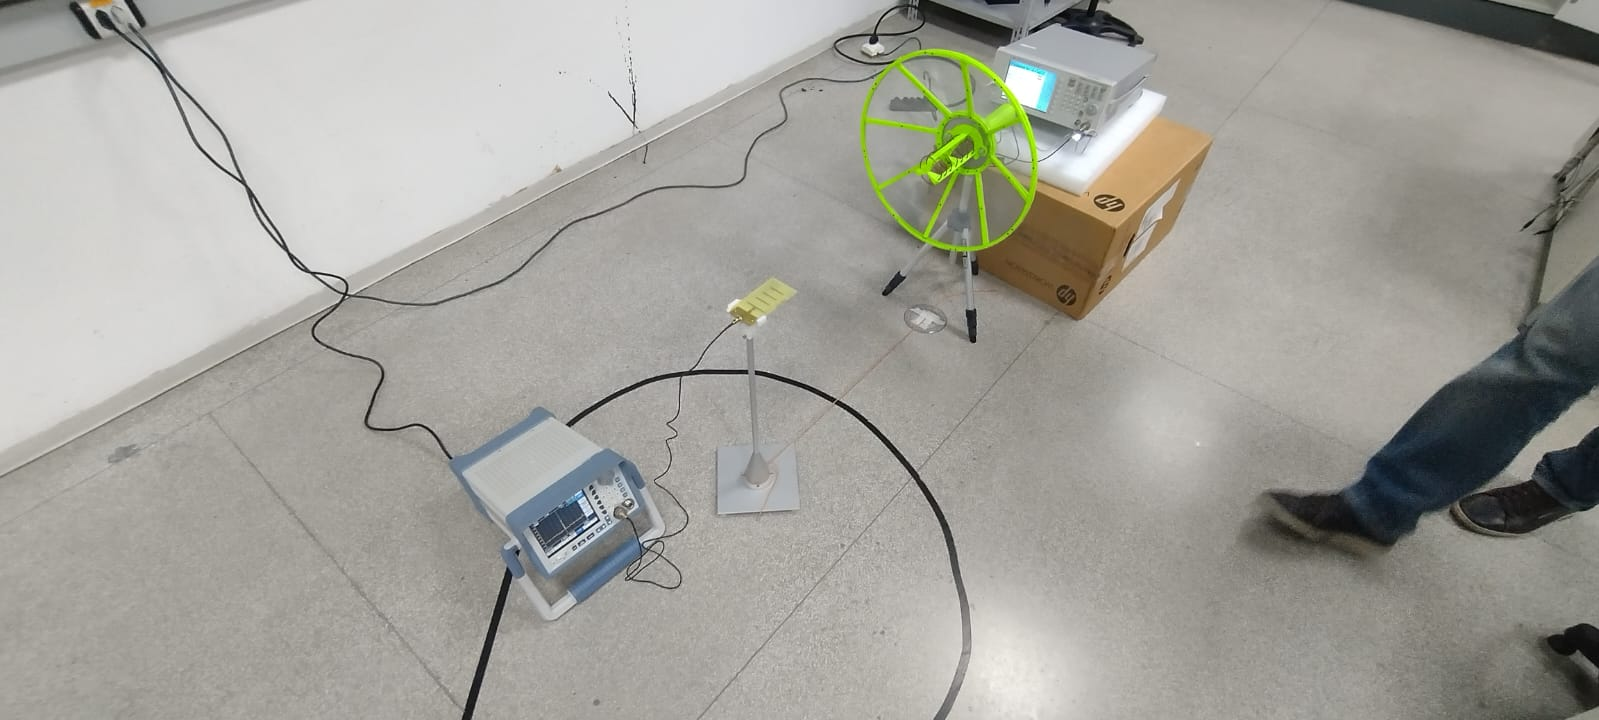
\includegraphics[width=1\textwidth]{figs/setup_completo_diagrama_rad.jpeg}
    \caption{Imagem com todos os equipamentos utilizados para o teste.}
    \legend{Fonte: Autor(2026)}
    \label{fig:todos_equipamentos_diagrama_radiacao}
\end{figure}
\begin{figure}[htbp]
    \centering
    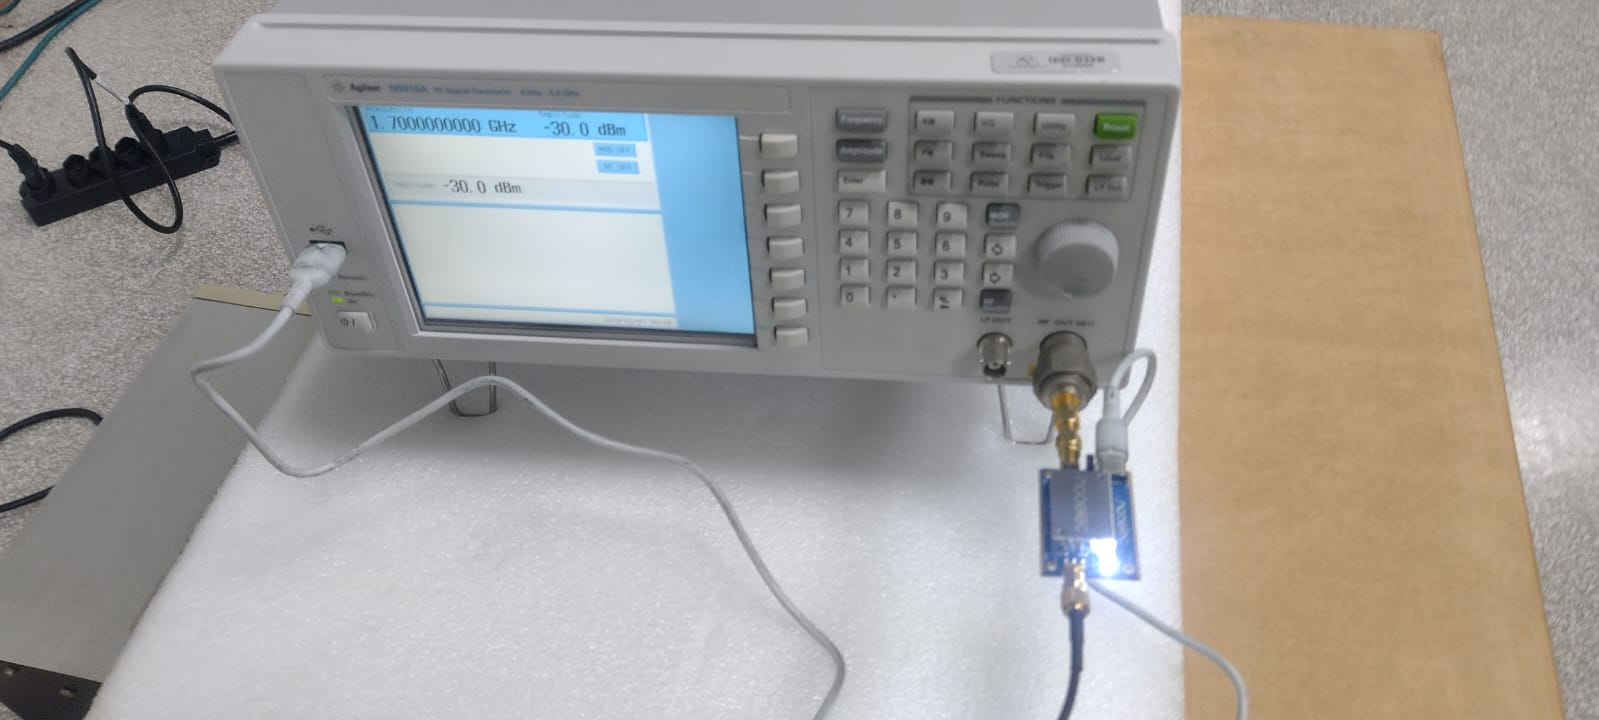
\includegraphics[width=1\textwidth]{figs/gerador_visor_teste_antena.jpeg}
    \caption{Configuração do gerador para o levantamento do diagrama de radiação.}
    \legend{Fonte: Autor(2026)}
    \label{fig:config_gerador_filtro}
\end{figure}
\begin{figure}[htbp]
    \centering
    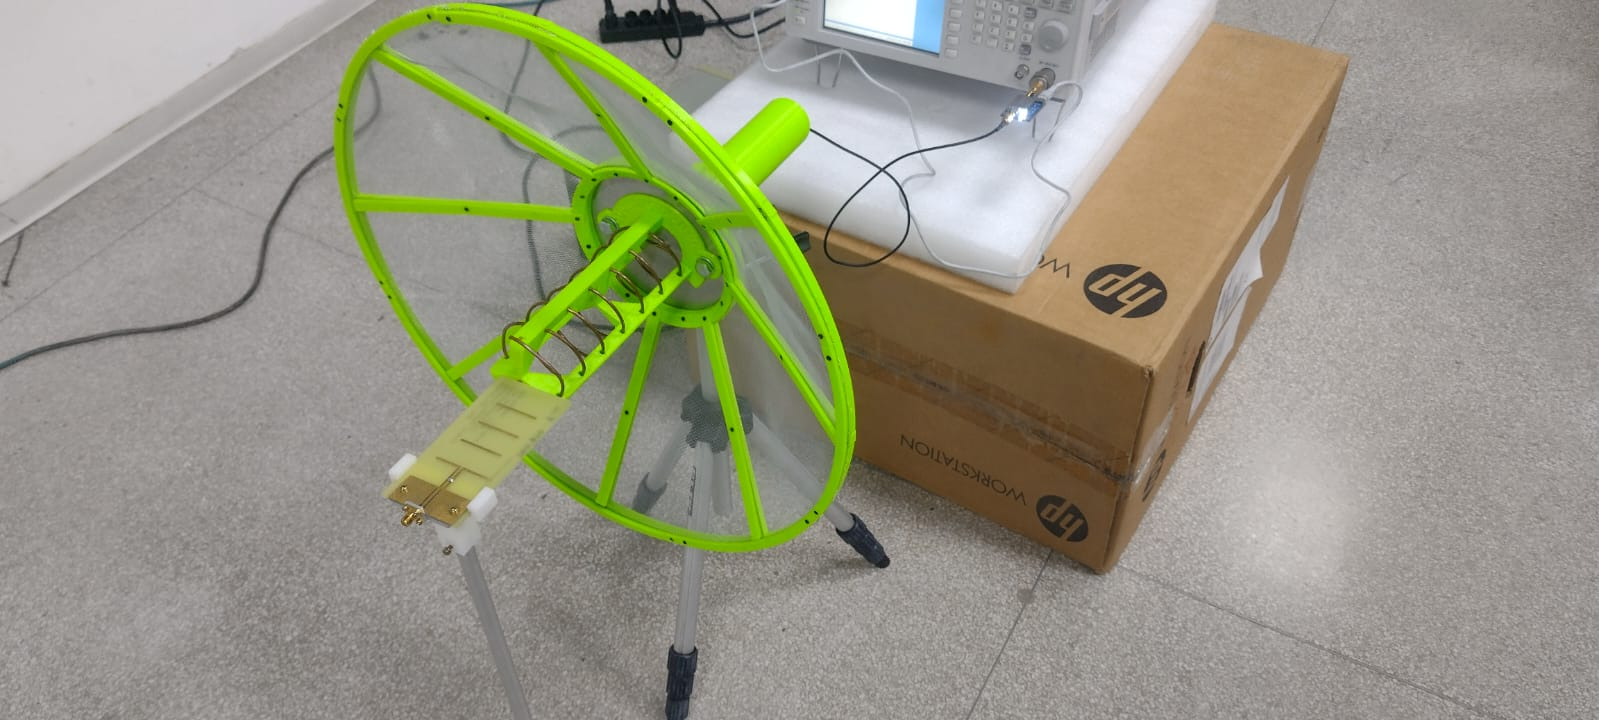
\includegraphics[width=1\textwidth]{figs/alinhamento_vertical_antenas.jpeg}
    \caption{Alinhamento das antenas no mesmo plano horizontal.}
    \legend{Fonte: Autor(2026)}
    \label{fig:alinhamento_antena_plano_horizontal}
\end{figure}
\begin{figure*}[htbp]
        \subfloat[Início da medição da distância entre as antenas]{%
            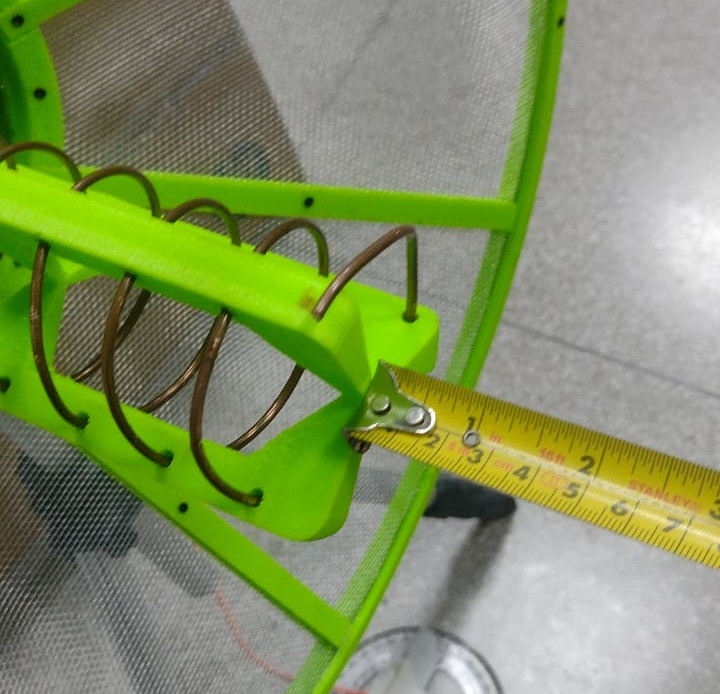
\includegraphics[width=0.8\linewidth]{figs/inicio_medicao_antena.jpeg}%
            \label{subfig:inicio_medicao}%
        }\\
        \subfloat[Final da medição da distância entre as antenas]{%
            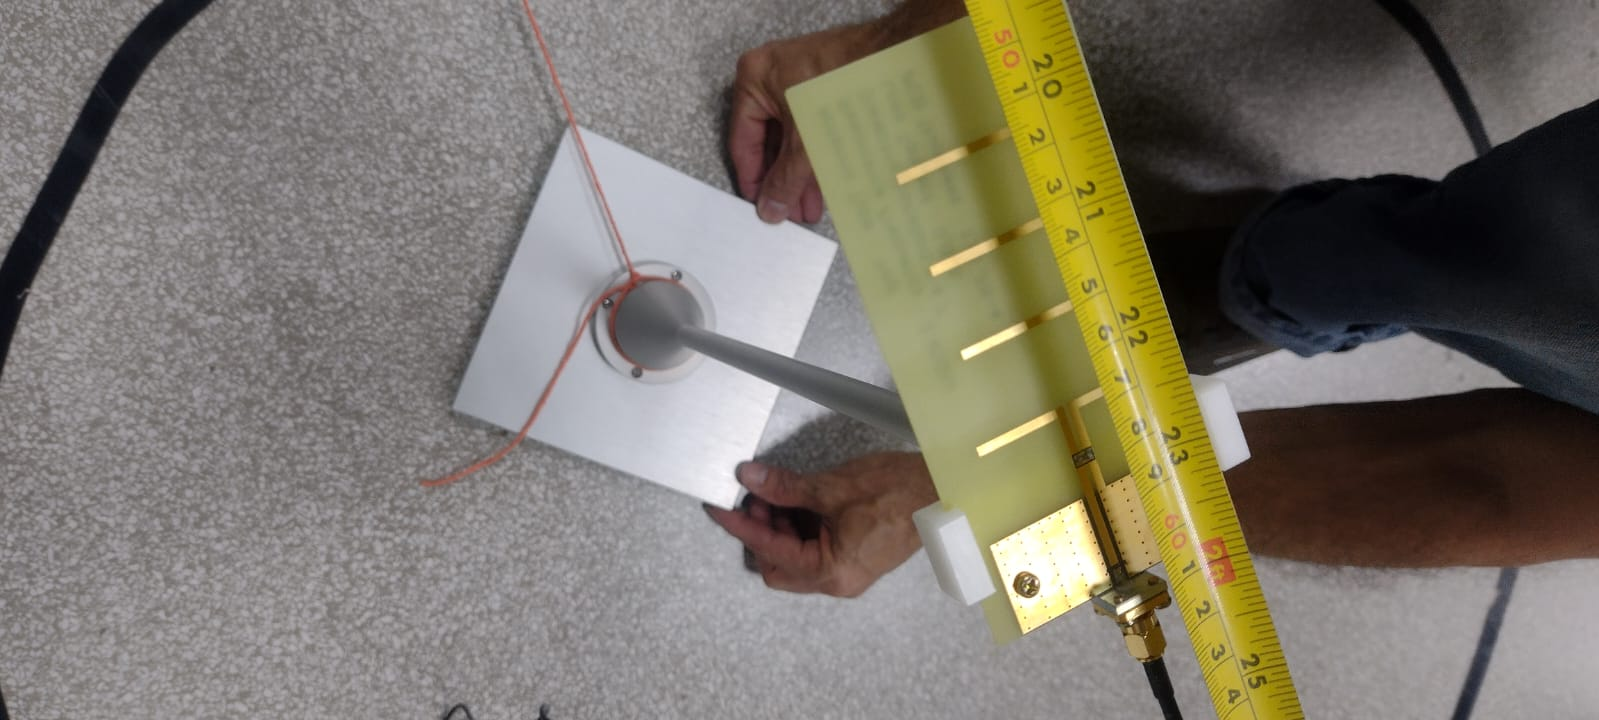
\includegraphics[width=0.8\linewidth]{figs/fim_medicao_antena.jpeg}%
            \label{subfig:fim_medicao}%
        }
        \caption{Medição da distância entre as antenas, de seu início na Figura \ref{subfig:inicio_medicao} até o final na Figura \ref{subfig:fim_medicao}.}
        \legend{Fonte: Autor (2026)}
        \label{fig:medicao_dist_antenas}
\end{figure*}

\begin{table}[htbp]
\centering
\caption{Comparação entre \texttt{Lado Esquerdo} e \texttt{Lado Direito} com passo de $\pm5^\circ$.}
\begin{tabular}{rrrr}
\toprule
\textbf{Ângulo ($^\circ$)} & \textbf{\texttt{Lado Esquerdo}} & \textbf{\texttt{Lado Direito}}\\
\midrule
0  & $-26.5$ & $-24.9$ \\
$\pm5$  & $-26.8$ & $-25.3$ \\
$\pm10$ & $-27.0$ & $-25.6$ \\
$\pm15$ & $-27.4$ & $-26.4$ \\
$\pm20$ & $-27.3$ & $-29.2$ \\
$\pm25$ & $-31.5$ & $-29.5$ \\
$\pm30$ & $-33.5$ & $-32.3$ \\
$\pm35$ & $-32.4$ & $-31.6$ \\
$\pm40$ & $-36.7$ & $-37.2$ \\
$\pm45$ & $-43.1$ & $-46.2$ \\
$\pm50$ & $-44.4$ & $-44.0$ \\
$\pm55$ & $-49.3$ & $-41.1$ \\
$\pm60$ & $-49.8$ & $-45.2$ \\
$\pm65$ & $-46.0$ & $-45.3$ \\
$\pm70$ & $-50.1$ & $-43.3$ \\
$\pm75$ & $-57.1$ & $-44.3$ \\
$\pm80$ & $-43.7$ & $-44.5$ \\
$\pm85$ & $-46.7$ & $-48.8$ \\
$\pm90$ & $-47.4$ & $-45.4$ \\
$\pm110$ & $-55.2$ & $-50.2$ \\
\bottomrule
\end{tabular}
\label{tab:dados_diag_rad}
\end{table}


\end{apendicesenv}
% ---